\documentclass[12pt,a4paper]{report}

% Packages
\usepackage[margin=1in,left=1.5in]{geometry}
\usepackage{times}
\usepackage{setspace}
\usepackage{titlesec}
\usepackage[nottoc,notlot,notlof]{tocbibind}
\usepackage{tocloft}
\usepackage{fancyhdr}
\usepackage{graphicx}
\usepackage{booktabs}
\usepackage{usecase}
\usepackage{xcolor}
\usepackage{hyperref}

% hide links so no color appear, but they still work
\hypersetup{
    hidelinks
}

% Page numbering
\pagenumbering{roman}

% Title formatting
\titleformat{\chapter}{\normalfont\huge\bfseries\uppercase}{\thechapter}{20pt}{\huge}

% Document begin
\begin{document}

% Title Page
\begin{titlepage}
    \begin{center}
        \vspace*{1cm}
        
\includegraphics[height=1cm]{images/yu-logo.png}\\[1cm]
        {\Large\bfseries AL YAMAMAH UNIVERSITY}\\[0.5cm]
        {\large College of Engineering and Architecture}\\[0.5cm]
        {\large Bachelor of Science in Software and Network Engineering}\\[2cm]
        {\Huge\bfseries 
            \begin{spacing}{1}
                Jadwal: An Elegant, iOS-based Calendar Manager
            \end{spacing}
        }
        \vspace{2cm}
        {\Large\bfseries Graduation Project}\\[2cm]
        \begin{center}
            \setlength{\fboxsep}{10pt}
            \setlength{\fboxrule}{1pt}
            \fbox{
                \begin{tabular}{p{0.45\linewidth}p{0.45\linewidth}}
                    \multicolumn{2}{c}{\textbf{Group Project Submission}} \\
                    \midrule
                    \textbf{Student Names} & \textbf{Student IDs} \\
                    \midrule
                    YAZED ALKHALAF & 202211123 \\
                    SAIMAN TAKLAS & 202021400 \\
                    AFFAN MOHAMMAD & 202211086 \\
                    ALI BA WAZIR & 202211018 \\
                    \midrule
                    \multicolumn{2}{l}{\textbf{Submission Date}: 19 Sep 2024} \\
                    \multicolumn{2}{l}{\textbf{Supervised By}: Dr. Inaya Allah} \\
                \end{tabular}
            }
        \end{center}
        \vfill
        {\large First Semester 2024--2025}
    \end{center}
\end{titlepage}

% Preface section
\chapter*{Abstract}
\addcontentsline{toc}{chapter}{Abstract}

\chapter*{Acknowledgment}
\addcontentsline{toc}{chapter}{Acknowledgment}
\newpage

\tableofcontents

\newpage
\listoffigures

\newpage
\listoftables
\newpage

\chapter*{List of Abbreviations}
\addcontentsline{toc}{chapter}{List of Abbreviations}

% Main body (switch to Arabic numerals)
\pagenumbering{arabic}

\chapter{Introduction}


\section{Background of the Study}

As the world is moving towards globalizing, effective time management is becoming very important. Considering how everything seems to be rushing in today's world, there is a high requirement for an effective user-friendly time management tool. Paper-based calendars have been used for addressing the complexities of managing multiple schedules across various aspects of life such as work, school, and personal commitments. However, they often fall short in providing a comprehensive solution to modern scheduling challenges.

The introduction of the digital calendar has somewhat solved this problem but still, users face a lot of issues in keeping their calendars up-to-date and synchronized. There are still few people that manually input events into their calendars. This could be really tiring, especially when dealing with multiple calendars.

Moreover, the rise of instant messaging platforms like WhatsApp has changed the way we communicate and plan events. Mostly, important dates and appointments are discussed informally leading to a disconnect between where the information is initially shared and where it needs to be recorded for effective time management.

To address these challenges, we are planning an application called \textit{Jadwal}, which aims to revolutionize how people manage their time and schedules in the digital age.

\section{Problem Statement}

Users often face challenges in keeping their calendars up-to-date, particularly when dealing with information from various sources, including informal communication mediums like WhatsApp. The process of manually adding events to the calendar is both time-consuming and prone to errors. Additionally, managing multiple calendars—such as those for work, school, and personal life—creates further complexity and increases the risk of scheduling conflicts. The lack of seamless integration with popular communication platforms exacerbates the problem, leading to a higher likelihood of missing important events due to the scattered distribution of information across different calendars and data sources.

\section{Objectives of the Study}

The main objectives of Jadwal are:

\begin{itemize}
    \item To develop an intelligent calendar management system that automatically extracts events from the communication channels and adds them to the user's main calendar.
    \item To create a user friendly interface that allows users to automatically add events to the calendar.
    \item To implement smart resolution system that notifies users of scheduling conflicts and provides easy options for resolution.
    \item To integrate all the calendars into Jadwal's single calendar view to make viewing and managing all the events easy.
    \item To prioritize and automatically schedule daily routines such as waking time, sleeping time and prayer time.
    \item To significantly reduce the time users spend on manual calendar management.
\end{itemize}

\section{Scope of the Study}

Jadwal is not just another calendar application; it's a comprehensive time management tool designed to aggregate and optimize your existing calendars and data sources. The scope of the project includes:

\begin{itemize}
    \item Development of an iOS application as the primary platform.
    \item Integration with calendars using CalDAV.
    \item WhatsApp message parsing for event extraction (subject to technical feasibility).
    \item Target audience: Busy professionals, students, and anyone juggling multiple schedules.
    \item User testing phase to ensure ease of use and effectiveness.
\end{itemize}

Our testing methods will include:
\begin{itemize}
    \item Beta testing with a diverse group of users.
    \item Analytics to track user behavior and app performance.
\end{itemize}

\section{Significance of the Study}

Jadwal endeavours to solve problems and its significance can be summarized in the following:

\begin{enumerate}
    \item \textbf{Time is Money}: Time is the only asset you can't get more of, it is being consumed til the last day of your life.
    \item \textbf{Prayer First Calendar}: Prayer times come first, then your daily scheduled items.
    \item \textbf{Streamlined Time Management}: By automatically extracting events from various communication channels, Jadwal significantly reduces the time and effort required for manual calendar management, allowing users to focus on more productive tasks.
    \item \textbf{Reduced Human Error}: Automated event extraction and addition to calendars minimize the risk of missing important events or appointments due to manual input errors or forgetfulness.
    \item \textbf{Integrated Communication and Scheduling}: By bridging the gap between informal communication (e.g., WhatsApp) and formal scheduling, Jadwal addresses a critical pain point in modern time management.
    \item \textbf{Conflict Resolution}: The smart resolution system helps users identify and resolve scheduling conflicts efficiently, reducing stress and improving overall time management.
    \item \textbf{Holistic View of Commitments}: By integrating multiple calendars into a single view, Jadwal provides users with a comprehensive overview of their commitments across various aspects of life, facilitating better decision-making and work-life balance.
\end{enumerate}

\section{Limitations of the Study}

Nothing is perfect, and our project is not a outlier. The limitations we have figured out about it are as follows:

\begin{itemize}
    \item WhatsApp integration allows the app to read the users messages, so it would be hard to prove privacy hasn't been breached.
    \item WhatsApp integration might not always be there, they are a third-party.
    \item Learning new technologies for iOS development might require more time than anticipated.
    \item Accuracy of our algorithms to detect keywords indicating an event agreement has happened, especially for languages other than English.
    \item Time and manpower constraints may limit the number of features we can implement.
    \item Dependency on third-party calendar APIs and their limitations.
\end{itemize}

\section{Organization of the Senior Project}

Our project plan can be illustrated in the following gantt chart, \textbf{Figure \ref{fig:project-gantt-chart}}.

\begin{figure}[!h]
    \centering
    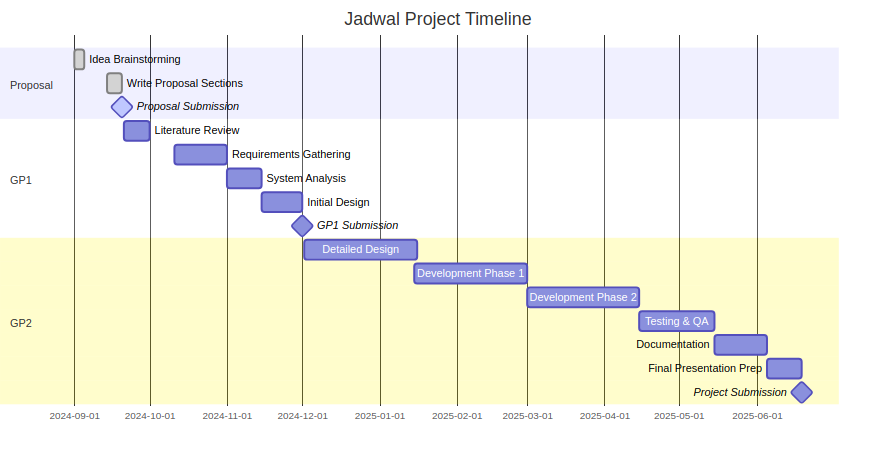
\includegraphics[width=\textwidth]{images/gantt.png}
    \caption{Project Gantt Chart}
    \label{fig:project-gantt-chart}
\end{figure}

\chapter{Literature Review}

In developing Jadwal, we have drawn inspiration from and built upon existing research and products in the field of intelligent calendar management. Some key references include:

\begin{itemize}
    \item \textbf{Clockwise (https://www.getclockwise.com/):} A smart calendar assistant that optimizes schedules and manages team coordination \cite{clockwise}. Clockwise's approach to intelligent time blocking and meeting optimization provides valuable insights for Jadwal's automated scheduling features.
    \item \textbf{Motion (https://www.usemotion.com/):} Motion's Intelligent Calendar takes your meetings, your tasks, your to-do list, your activities, and creates one perfect, optimized schedule to get it all done \cite{motion}.
    \item \textbf{Reclaim AI (https://reclaim.ai/):} An intelligent time management tool that helps optimize schedules and automate tasks \cite{reclaim}.
    \item \textbf{Calendi (https://calendi.ai/):} Calendi describes itself as: ``Calendi is an AI calendar system. Use it for scheduling tasks, automating meetings, and witness the future of calendar.'' \cite{calendi}
    \item \textbf{An Exploratory Study of Calendar Use:} ``Prospective remembering is the use of memory for remembering to do things in the future, as different from retrospective memory functions such as recalling past events.'' \cite{tungare2008exploratorystudycalendaruse}
    \item \textbf{WhatsApp Integration:} Our research indicates that direct WhatsApp integration for event extraction has not been widely implemented in existing calendar applications, making this a unique feature of Jadwal.
\end{itemize}

\begin{figure}[!h]
    \centering
    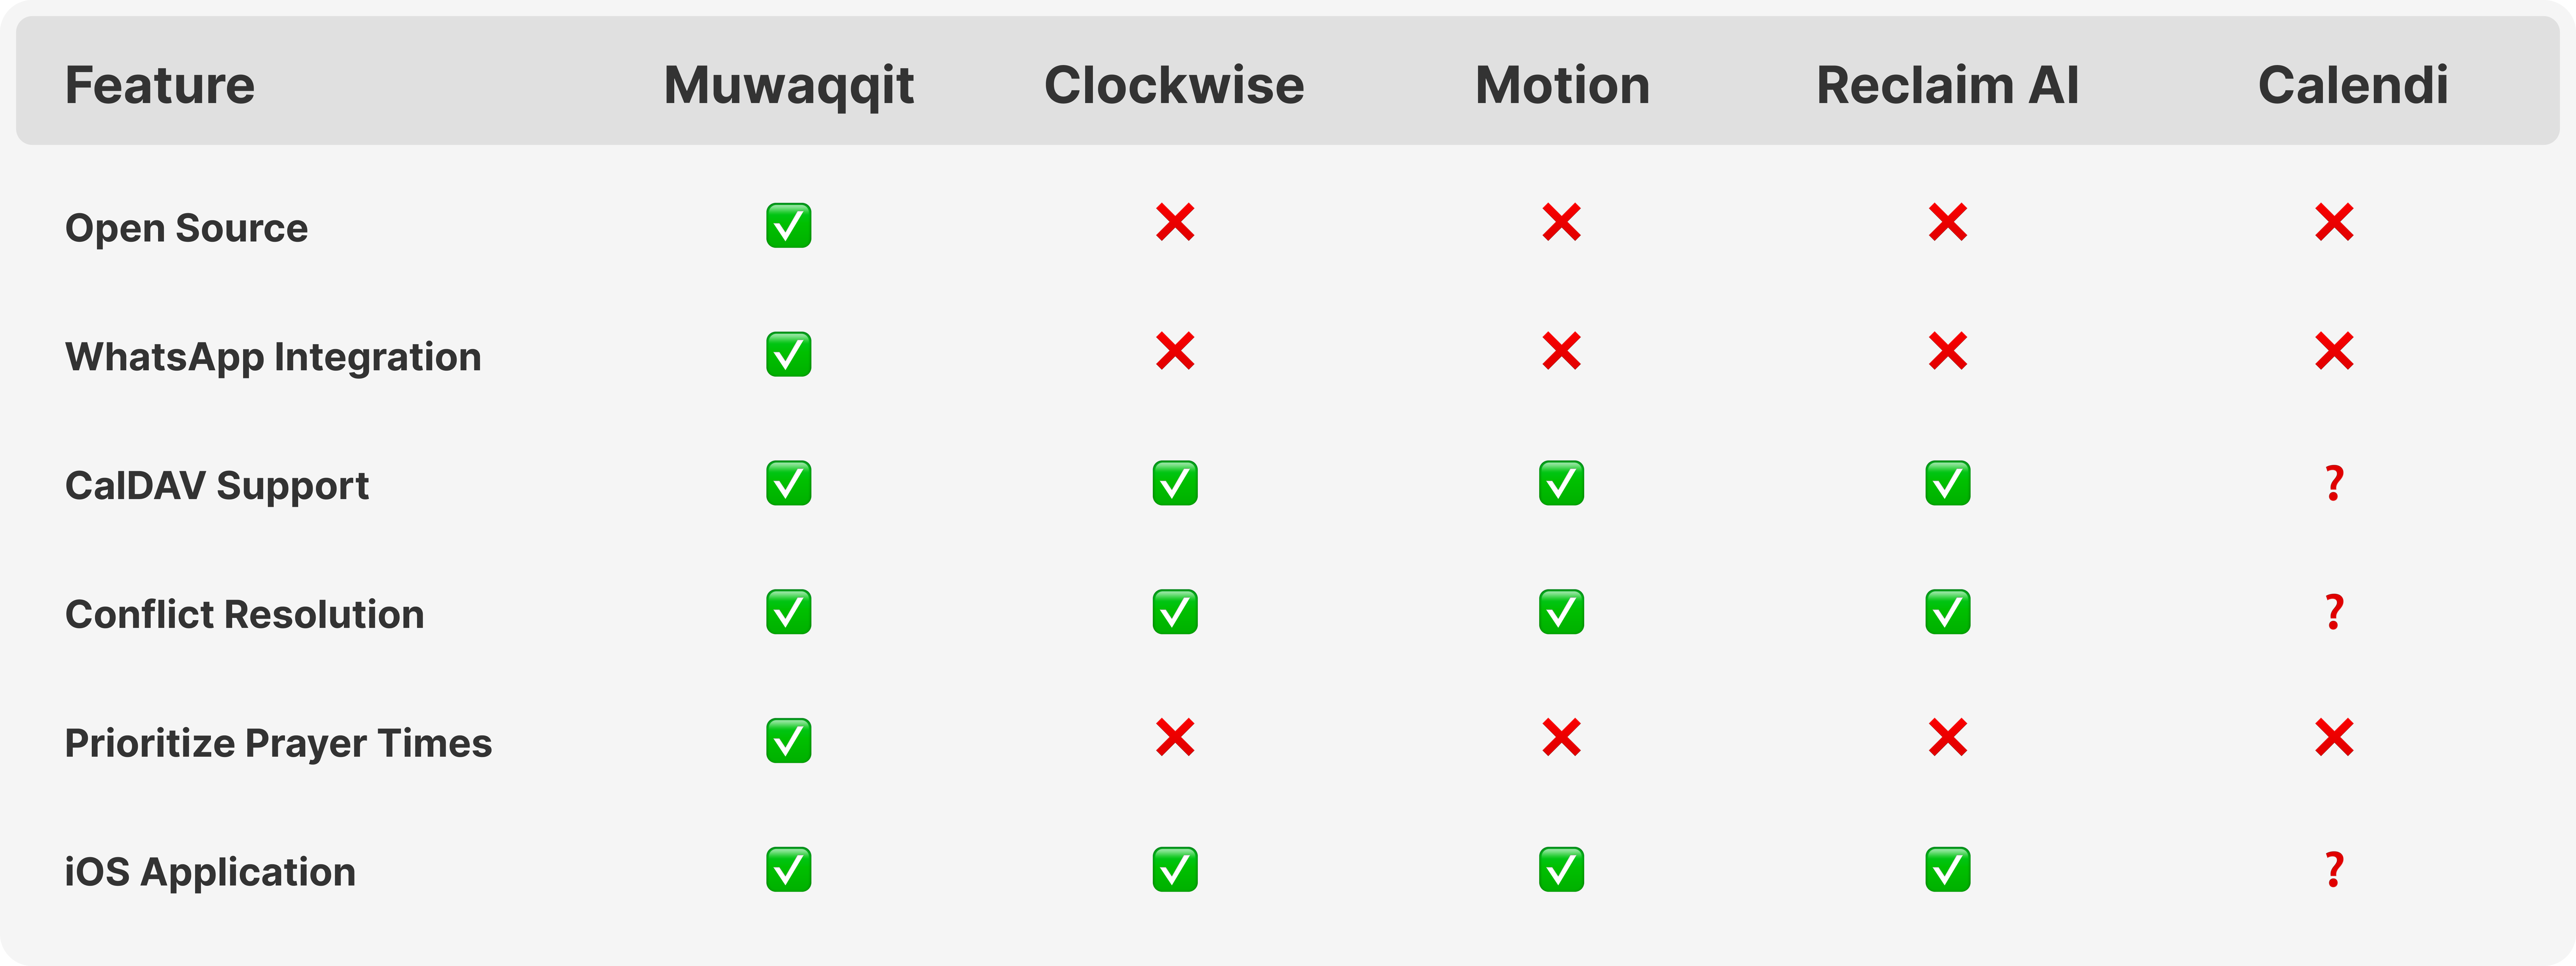
\includegraphics[width=\textwidth]{images/features-table.png}
    \caption{Feature Comparison Table}
    \label{fig:features-table}
\end{figure}

\chapter{System Analysis and Design}

\section{Functional Requirements}

\begin{itemize}
    \item The user shall be able to access their account using either Google OAuth or magic link via Email. For new users, a new accout is created, and for existing users, they are given access to their account directly
    \item The system shall send a welcome email to new users.
    \item The user should be able to connect a calendar using CalDAV.
    \item The user should be able to connect their WhatsApp account.
    \item The user should be able to add events manually and set priorities optionally.
    \item The user should be able to view integrated calendar.
    \item The user should be able to configure daily routines.
    \item The user should be able to manage scheduling conflicts.
    \item The user should be able to schedule prayer times.
    \item The system shall send event notifications to the user.
    \item The system shall personalize the experience based on answers provided by the users.
    \item The system shall add the WhatsApp extracted events to the calendar. If a conflict occurs, the user shall get a notification to resolve the conflict with suggestions.
    \item The system shall synchronize calendar data across multiple devices.
\end{itemize}

\section{Non-Functional Requirements}

\begin{itemize}
    \item \textbf{Platform Compatibility:} The app shall be compatible with iOS devices running iOS 14.0 or later.
    \item \textbf{Performance:} The app shall load the main calendar view within 3 seconds on 5G with speeds above 200mpbs.
    \item \textbf{User Experience:} The user interface shall follow iOS Human Interface Guidelines for consistency and ease of use.
    \item \textbf{Security:} All data transmissions between the app and servers shall be encrypted using HTTPS.
    \item \textbf{Localization:} The app shall support localization in Arabic and English.
    \item \textbf{Data Privacy:} The app shall comply with the data protection regulations and laws in Saudi Arabia.
\end{itemize}

\section{System use-cases}

\textbf{Figure \ref{fig:use-case-diagram}} shows the use case diagram for the system of Jadwal.

\begin{figure}[!h]
    \centering
    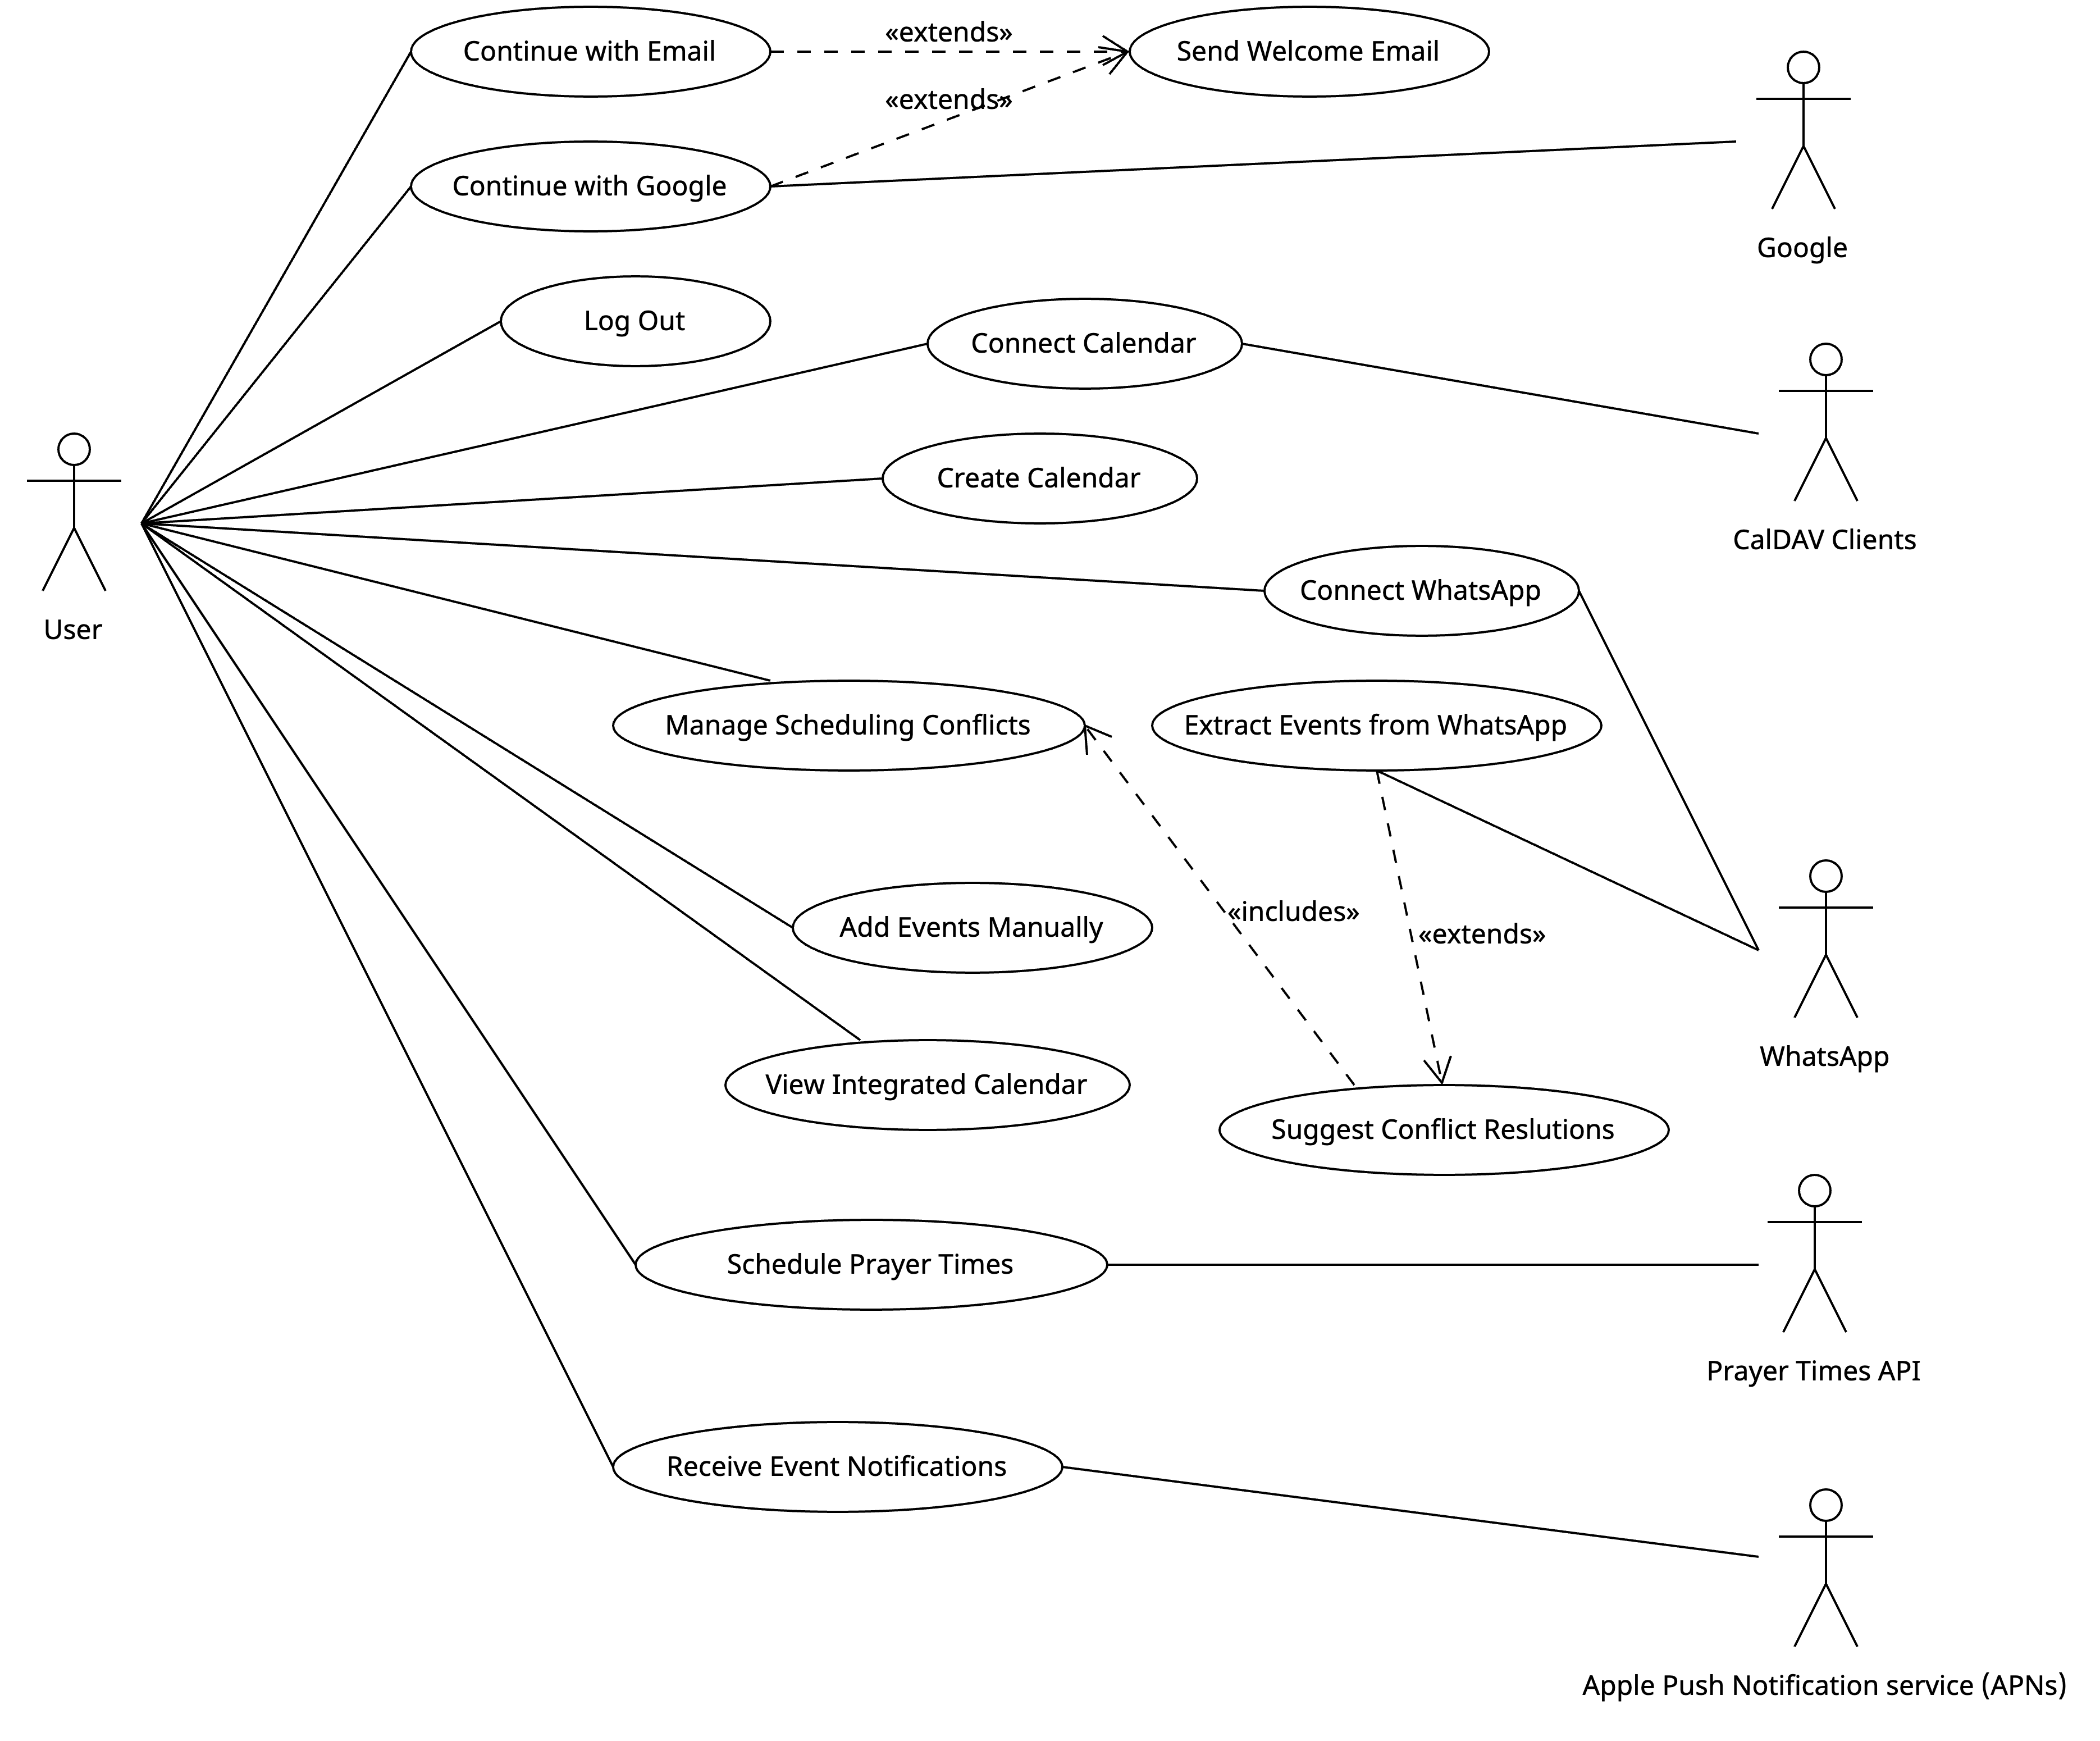
\includegraphics[width=\textwidth]{images/use-case-diagram.png}
    \caption{Use Case Diagram of Jadwal}
    \label{fig:use-case-diagram}
\end{figure}

\begin{usecase}{Continue with Email}
  \ucbasicinfo{High}{Regular}
  \ucshortdescription{This UC allows users to login or create an account using their email.}
  \uctrigger{This UC starts when the user enters their email to the system.}
  \ucactors{User}{None}
  \ucpreconditions{User must have an email}
  \ucrelationships{Send Welcome Email}{N/A}{N/A}
  \ucinputsoutputs{
    \begin{itemize}
      \item \textbf{Email} (Source: User)
      \item \textbf{Magic Link (from email)} (Source: User)
    \end{itemize}
  }{
    \begin{itemize}
      \item \textbf{Magic link email} (Destination: User)
      \item \textbf{Confirmation messages} (Destination: User Interface)
      \item \textbf{JWT} (Destination: App)
    \end{itemize}
  }
  \ucmainflow{
    \begin{enumerate}
      \item The user enters their email.
            \ucinfo{System displays an email input field.}
      \item System creates an account if the user has no account, and then generates and sends the magic link.
            \ucinfo{App displays ``Check your email'' message.}
      \item The user clicks the magic link in the email.
            \ucinfo{The app is opened on the device of the user.}
      \item The app sends the token to the system to log the user in.
            \ucinfo{System verifies token and logs user in.}
    \end{enumerate}
  }
  \ucalternateflows{
    \begin{itemize}
      \item The user cancels the authentication request.
    \end{itemize}
  }
  \ucexceptions{
    \begin{itemize}
      \item Invalid email format.
      \item Magic link token expired or invalid.
      \item \textbf{Request sending failure}: If sending the request fails due to network issues, the system prompts the user to try again.
    \end{itemize}
  }
  \ucconclusion{This UC ends when the user is logged in.}
  \ucpostconditions{The system generates a JWT.}
  \ucspecialrequirements{An email server must be present to send magic link email.}
\end{usecase}

\begin{figure}[!h]
  \centering
  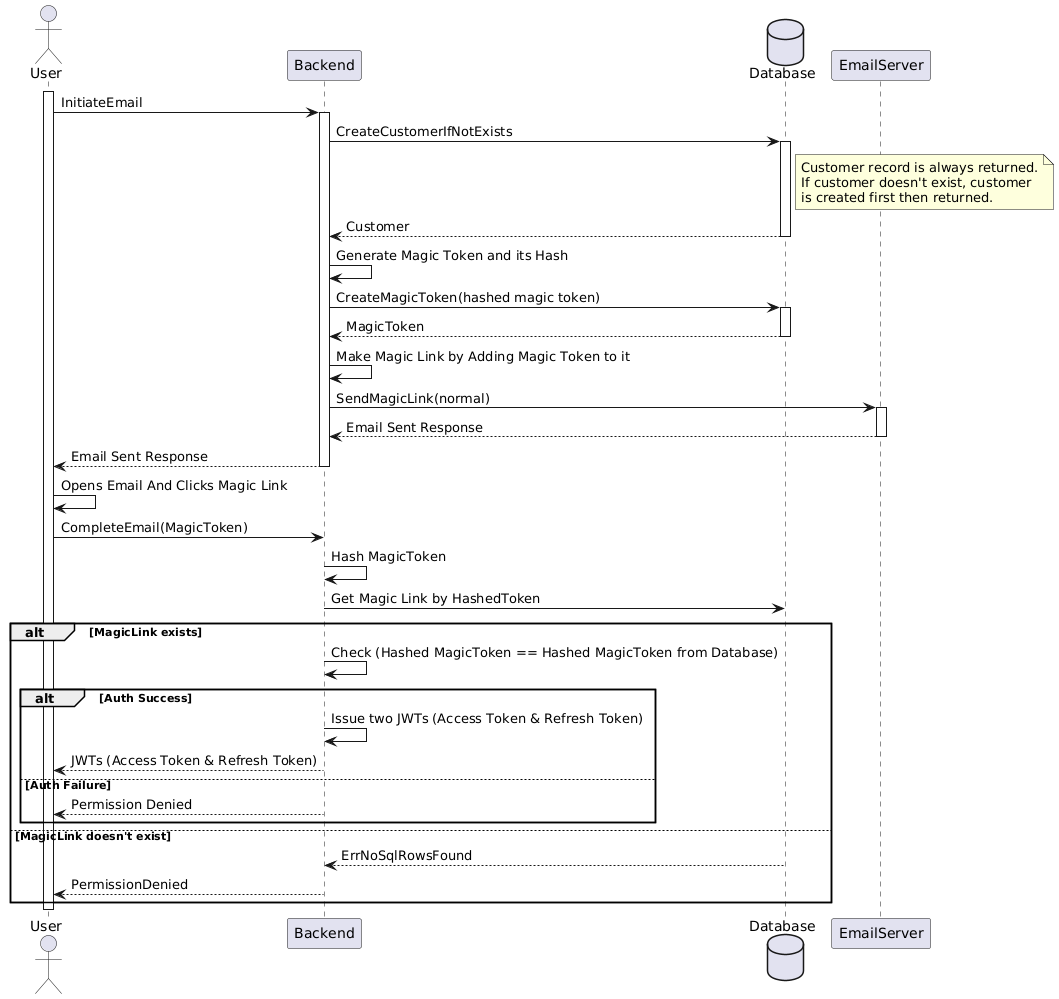
\includegraphics[width=\textwidth]{images/docs/diagrams/sequence-diagrams/all-sequence-diagrams/Continue with Email.png}
  \caption{Continue with Email Sequence Diagram}
  \label{fig:seq/continue-with-email}
\end{figure}

The "Continue with Email Sequence Diagram", shown in \textbf{Figure~\ref{fig:seq/continue-with-email}}, illustrates the process of email-based magic link authentication, involving interactions between the User, Backend, Database, and EmailServer. The process begins when the user initiates an action, such as signing up or logging in. The backend executes the CreateCustomerIfNotExists function to retrieve an existing customer record or create a new one if none exists. Once the customer is identified, the backend generates a magic token and its hashed version using the GenerateMagicToken function. The hashed token is stored in the database, and a magic link containing the token is created. The backend then sends the magic link to the user's email using the SendEmail function via the email server. The user clicks the magic link, triggering the CompleteFlow(MagicToken) request to the backend, where the provided token is validated against the stored hashed token in the database. If the tokens match, authentication succeeds, and the backend issues a JSON Web Token (JWT) to the user for future access. In cases where the token is invalid, expired, or the customer record is missing, the system responds with appropriate errors, such as PermissionDenied or EntryNotFound. This diagram demonstrates a secure flow for handling authentication via email magic links.
\begin{usecase}{Continue with Google}
  \ucbasicinfo{High}{Regular}
  \ucshortdescription{This UC allows users to login or sign up with their Google account.}
  \uctrigger{This UC starts when the user clicks ``Continue with Google'' button in the app.}
  \ucactors{User}{Google}
  \ucpreconditions{The user must have an active Google account.}
  \ucrelationships{Send Welcome Email}{N/A}{N/A}
  \ucinputsoutputs{
    \begin{itemize}
      \item \textbf{Google access token} (Source: User)
    \end{itemize}
  }{
    \begin{itemize}
      \item \textbf{Authentication response} (Destination: User)
      \item \textbf{JWT} (Destination: App)
    \end{itemize}
  }
  \ucmainflow{
    \begin{enumerate}
      \item The user click continue with Google.
        \ucinfo{App uses OAuth to authenticate with Google}
      \item App sends Google access token to the system.
        \ucinfo{System verifies the token is issued for us and then issues JWT for usage within the app.}
    \end{enumerate}
  }
  \ucalternateflows{
    \begin{itemize}
      \item The user cancels the authentication request.
    \end{itemize}
  }
  \ucexceptions{
    \begin{itemize}
      \item Google access token invalid or expired.
      \item \textbf{Request sending failure}: If sending the request fails due to network issues, the system prompts the user to try again.
    \end{itemize}
  }
  \ucconclusion{This UC ends when the user is logged in.}
  \ucpostconditions{The system generates a JWT.}
  \ucspecialrequirements{A google client must be present for the validation of the access token to be possible.}
\end{usecase}

\begin{figure}[!h]
  \centering
  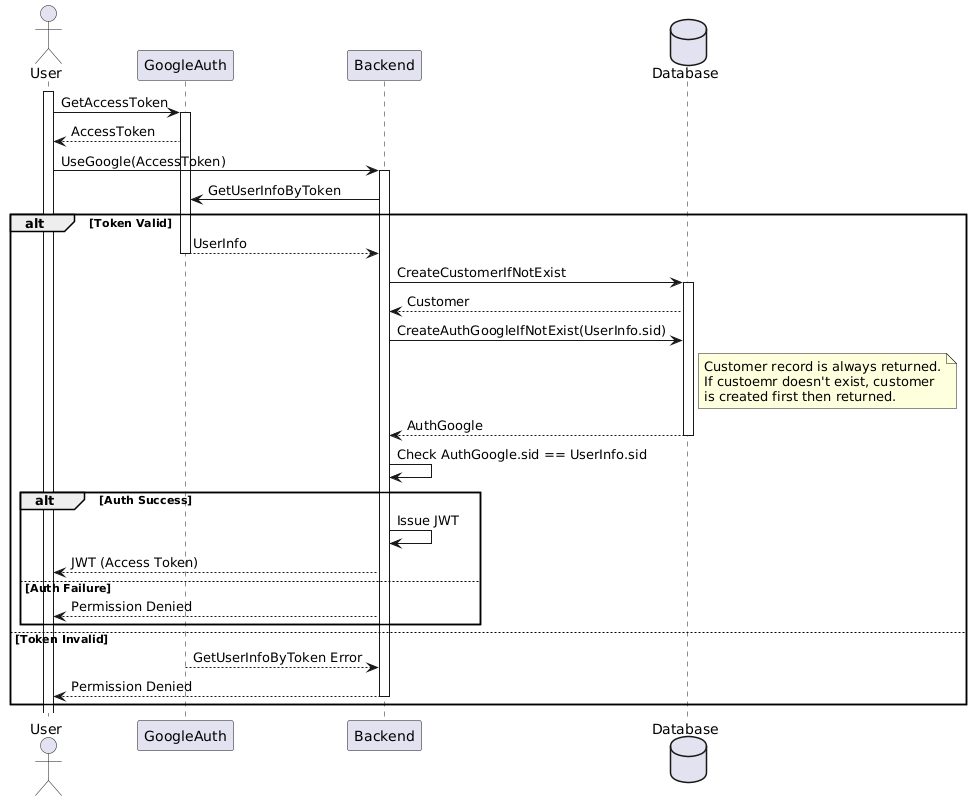
\includegraphics[width=\textwidth]{images/docs/diagrams/sequence-diagrams/all-sequence-diagrams/Continue with Google.png}
  \caption{Continue with Google Sequence Diagram}
  \label{fig:seq/continue-with-google}
\end{figure}
\begin{usecase}{Send Welcome Email}
    \ucbasicinfo{Low}{Regular}
    \ucshortdescription{This UC welcomes the user to the platform.}
    \uctrigger{This UC starts when the user account is created.}
    \ucactors{User}{None}
    \ucpreconditions{User account must be created in the system.}
    \ucrelationships{N/A}{N/A}{N/A}
    \ucinputsoutputs{
      \begin{itemize}
        \item \textbf{User name} (Source: System)
        \item \textbf{Welcome email template} (Source: System)
      \end{itemize}
    }{
      \begin{itemize}
        \item \textbf{Welcome email} (Destination: User)
      \end{itemize}
    }
    \ucmainflow{
      \begin{enumerate}
        \item The system fetches the user information.
          \ucinfo{The database is used.}
        \item The system fetches the send welcome email template.
          \ucinfo{The template is filled with the user name.}
        \item The system sends the email with the template.
          \ucinfo{The email is received by the user welcoming them.}
      \end{enumerate}
    }
    \ucexceptions{
      \begin{itemize}
        \item Email server is down.
      \end{itemize}
    }
    \ucconclusion{This UC ends when the user receives an email from us welcoming them.}
    \ucspecialrequirements{An email server must be present to send welcome email.}
\end{usecase}

\begin{figure}[!h]
  \centering
  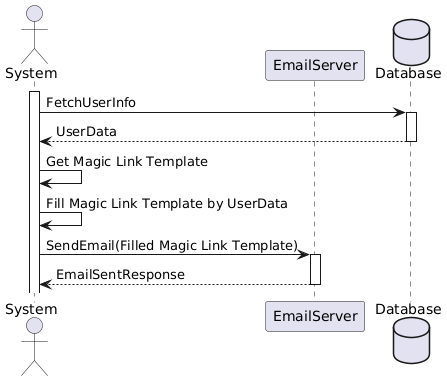
\includegraphics[width=\textwidth]{images/docs/diagrams/sequence-diagrams/all-sequence-diagrams/Send Welcome Email.png}
  \caption{Send Welcome Email Sequence Diagram}
  \label{fig:seq/send-welcome-email}
\end{figure}
\begin{usecase}{Continue with Google}
  \ucbasicinfo{\#2}{HIGH}{Regular}
  \ucshortdescription{This UC allows users to login or continue with Google if we have a Google account}
  \uctrigger{This UC starts when the user enters their email to the system.}
  \ucactors{User}{Google}
  \ucpreconditions{User must have an activated or valid Google email.}
  \ucrelationships{Send Welcome Email}{N/A}{N/A}
  \ucinputsoutputs{
    \begin{itemize}
      \item \textbf{Google account} (Source: User)
      \item \textbf{Authentication request to Google} (Source: System)
    \end{itemize}
  }{
    \begin{itemize}
      \item \textbf{Success or error message} (Destination: User)
      \item \textbf{Authentication response} (Destination: Google)
    \end{itemize}
  }
  \ucmainflow{
    \begin{enumerate}
      \item The user click continue with Google.
        \ucinfo{System displays "continue with Google" button}
      \item Authentication request.
        \ucinfo{A request sent to Google for user authentication and get JWT and sent it to the system, while the system will generate a our JWT}
      \item Authentication response.
        \ucinfo{Confirmation of successful authentication}
    \end{enumerate}
  }
  \ucalternateflows{
    \begin{itemize}
      \item User cancels authentication
      \item Authentication failure
    \end{itemize}
  }
  \ucexceptions{
    \begin{itemize}
      \item Invalid Google email
      \item Network issue
    \end{itemize}
  }
  \ucconclusion{}
  \ucpostconditions{The user is successfully authenticated and redirected to the main application interface}
  \ucbusinessrules{
    \begin{itemize}
      \item User should have valid Google account
    \end{itemize}
  }
  \ucspecialrequirements{Sign-in page should display clear button and error message}
\end{usecase}
\begin{usecase}{Connect Calendar}
    \ucbasicinfo{Medium}{Regular}
    \ucshortdescription{This UC allows the user to access their iOS device calendars through EventKit and configure CalDAV accounts.}
    \uctrigger{This UC is triggered when the user first launches the app or manually initiates calendar access.}
    \ucactors{User}{EventKit}
    \ucpreconditions{User must be logged in}
    \ucrelationships{N/A}{N/A}{N/A}
    \ucinputsoutputs{
        \begin{itemize}
            \item \textbf{Calendar Access Permission} (Source: User)
            \item \textbf{CalDAV Account Credentials} (Source: Backend)
        \end{itemize}
    }{
        \begin{itemize}
            \item \textbf{Local Calendar Access Status} (Destination: System)
            \item \textbf{Calendar Events} (Destination: App)
        \end{itemize}
    }
    \ucmainflow{
        \begin{enumerate}
            \item The system requests calendar access permission from the user.
                  \ucinfo{The app requests EventKit authorization to access device calendars.}
            \item The system retrieves CalDAV account credentials from the backend.
                  \ucinfo{The app fetches encrypted credentials for our CalDAV server.}
            \item The system configures CalDAV accounts through iOS's native calendar system.
                  \ucinfo{EventKit handles direct communication with all CalDAV servers (both ours and external ones).}
            \item The system fetches calendar events using EventKit.
                  \ucinfo{Events are fetched from all configured calendar accounts through iOS's native calendar system.}
            \item The system sets up local notifications for calendar events.
                  \ucinfo{Notifications are scheduled locally based on event reminders.}
        \end{enumerate}
    }
    \ucalternateflows{
        \begin{enumerate}
            \item If calendar access is denied, the user can grant permission through device settings.
            \item If account configuration fails, the user can retry the connection through iOS settings.
        \end{enumerate}
    }
    \ucexceptions{
        \begin{itemize}
            \item Calendar access permission denied
            \item Network issue retrieving account credentials
            \item iOS calendar account configuration failure
        \end{itemize}
    }
    \ucconclusion{The UC ends when the user has access to their device calendars and CalDAV accounts are configured in iOS.}
    \ucpostconditions{The app can read calendar events through EventKit from all configured calendar sources.}
    \ucspecialrequirements{The system must rely on iOS's native calendar system for all CalDAV communication.}
\end{usecase}

\begin{figure}[!h]
    \centering
    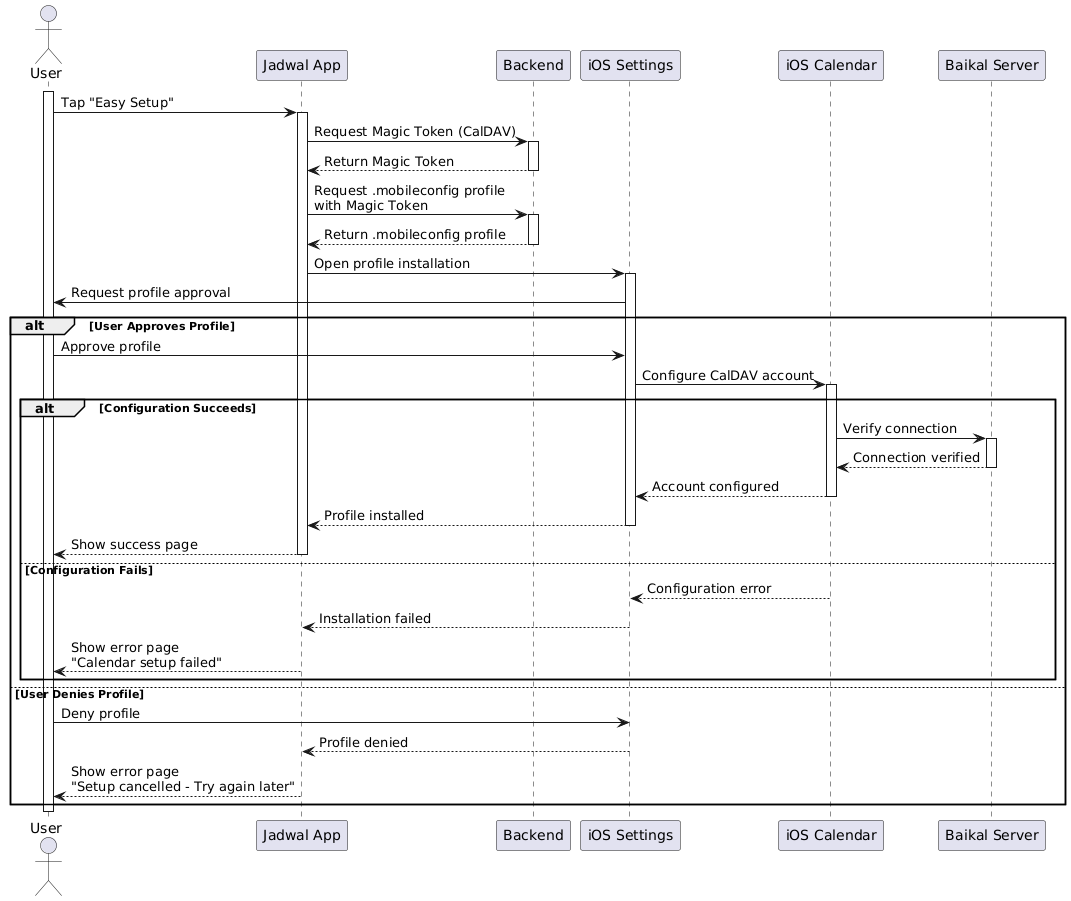
\includegraphics[width=\textwidth]{images/docs/diagrams/sequence-diagrams/all-sequence-diagrams/Connect Calendar.png}
    \caption{Connect Calendar Sequence Diagram}
    \label{fig:seq/connect-calendar}
\end{figure}

The ``Connect Calendar Sequence Diagram'', shown in \textbf{Figure~\ref{fig:seq/connect-calendar}}, illustrates the calendar integration process:

\begin{enumerate}
    \item \textbf{Local Calendar Access:} The iOS app uses EventKit framework to request and manage access to the device's calendars. This provides direct access to the user's existing calendar data.

    \item \textbf{Account Configuration:} The app retrieves encrypted CalDAV account credentials from the backend and uses iOS's native calendar system to configure the accounts. EventKit and iOS handle all direct communication with CalDAV servers, both our own and external ones.
\end{enumerate}

The Backend's role is strictly limited to securely storing and providing encrypted CalDAV account credentials. All calendar data synchronization, CalDAV communication, and event management happens through iOS's native calendar system using EventKit. This approach leverages iOS's built-in CalDAV client capabilities, ensuring reliable calendar synchronization while maintaining security of sensitive credentials.
// create calendar
\begin{usecase}{Connect WhatsApp}
  \ucbasicinfo{Medium}{Regular}
  \ucshortdescription{This UC allows the user to connect their WhatsApp account to the system.}
  \uctrigger{This UC is triggered when the user clicks on ``Connect WhatsApp'' button in the app.}
  \ucactors{User}{WhatsApp}
  \ucpreconditions{User must be logged in}
  \ucrelationships{N/A}{N/A}{N/A}
  \ucinputsoutputs{
    \begin{itemize}
      \item \textbf{WhatsApp phone number} (Source: User)
      \item \textbf{WhatsApp linking code} (Source: User)
    \end{itemize}
  }{
    \begin{itemize}
      \item \textbf{WhatsApp auth credentials} (Destination: System)
    \end{itemize}
  }
  \ucmainflow{
    \begin{enumerate}
      \item The user clicks ``Connect WhatsApp'' button.
            \ucinfo{The system asks for the user's WhatsApp phone number.}
      \item The user enters their WhatsApp phone number.
            \ucinfo{WhatsApp shows the linking code in their app.}
      \item The user enters the linking code in our app.
            \ucinfo{The app shows a success screen if connection was sucessful.}
    \end{enumerate}
  }
  \ucalternateflows{
    \begin{itemize}
      \item If the WhatsApp connection fails, the user must redo the steps and try again.
      \item If the user enters a wrong linking code, the connection of the WhatsApp account will fail unless they enter the correct code.
    \end{itemize}
  }
  \ucexceptions{
    \begin{itemize}
      \item \textbf{Wrong linking code:} If the user enters a wrong linking code too many times, the connection of the WhatsApp account will fail.
      \item \textbf{Network issue:} A network issue interrupting the communication between the app, the server, and WhatsApp.
    \end{itemize}
  }
  \ucconclusion{The UC ends when the user has a connected WhatsApp account in the system.}
  \ucpostconditions{The system has access to the user's WhatsApp account.}
\end{usecase}

\begin{figure}[!h]
  \centering
  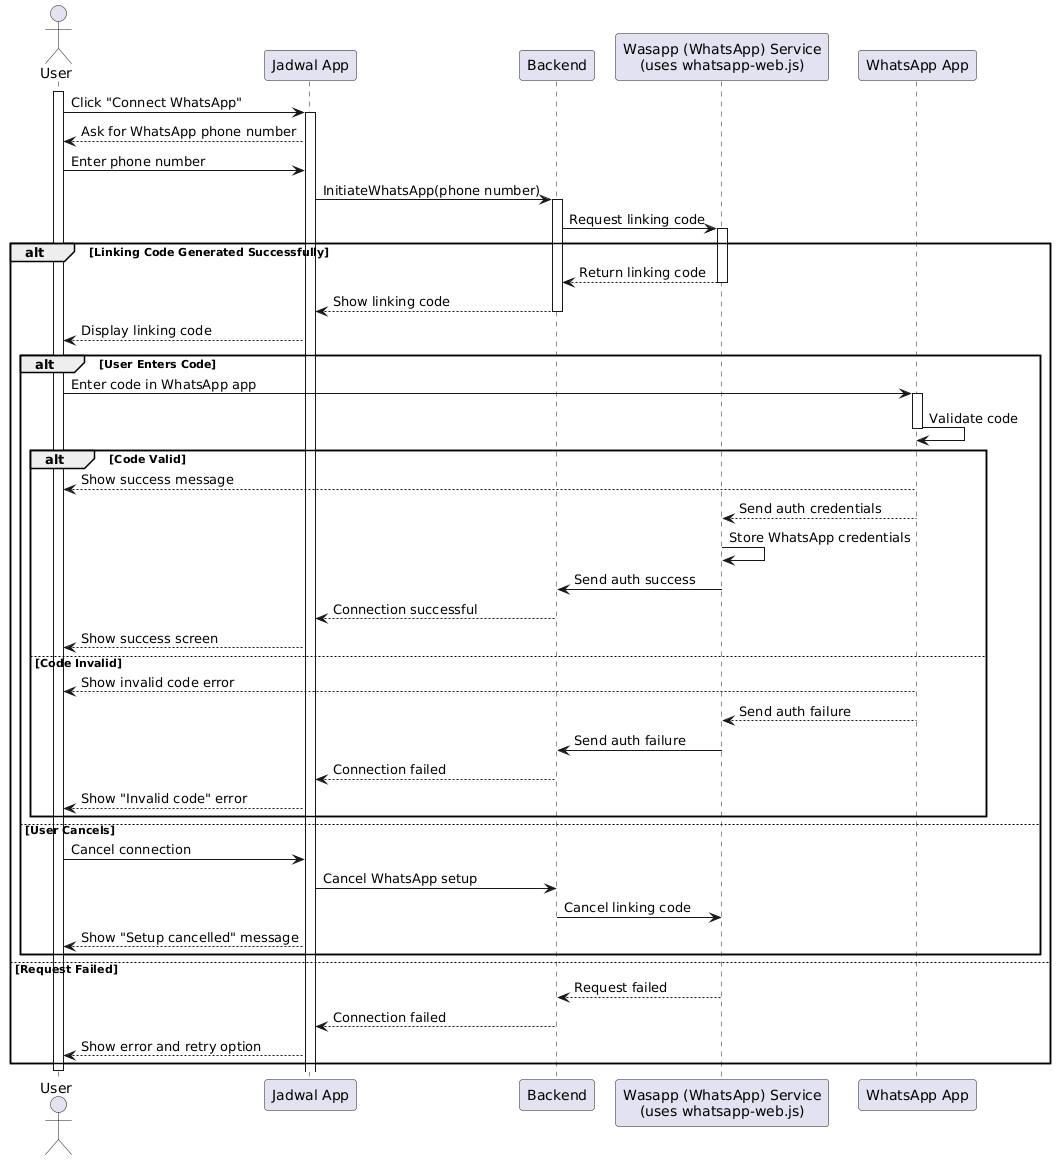
\includegraphics[width=\textwidth]{images/docs/diagrams/sequence-diagrams/all-sequence-diagrams/Connect WhatsApp.png}
  \caption{Connect WhatsApp Sequence Diagram}
  \label{fig:seq/connect-whatsapp}
\end{figure}

The "Connect WhatsApp Sequence Diagram", shown in \textbf{Figure~\ref{fig:seq/connect-whatsapp}}, illustrates the two-phase authentication process for connecting a user's WhatsApp account to Jadwal. The sequence begins with the InitiateWhatsApp gRPC call, where the user provides their phone number to the Backend.

The Backend then communicates with the WhatsApp service to request a linking code. This interaction follows two possible paths:

\begin{itemize}
  \item If the linking code request succeeds:
        \begin{enumerate}
          \item The user receives the linking code in their WhatsApp application
          \item The user initiates the CompleteWhatsApp gRPC call with the linking code
          \item The Backend validates the code with WhatsApp
          \item Upon successful validation, the WhatsApp authentication credentials are securely stored in the Database for future use
        \end{enumerate}
  \item If the linking code request fails:
        \begin{itemize}
          \item The Backend immediately returns an InitiateWhatsApp failure response to the user
        \end{itemize}
\end{itemize}

During the completion phase, if the linking code validation fails, the Backend returns a CompleteWhatsApp failure response, requiring the user to restart the process. This secure two-phase authentication ensures that only legitimate WhatsApp account owners can connect their accounts to Jadwal while maintaining the integrity of the WhatsApp integration.
// extract events from whatsapp
\begin{usecase}{Suggest Conflict Resolutions}
  \ucbasicinfo{HIGH}{Regular}
  \ucshortdescription{This UC gives the user all the conflicts and possible ways to resolve it.}
  \uctrigger{The UC is triggered when a conflict is detected between any overlapping event}
  \ucactors{User}{Calendar System, WhatsApp}
  \ucpreconditions{The calendar must have events}
  \ucrelationships{None}{Manage Scheduling Conflicts}{None}
  \ucinputsoutputs{
    \begin{itemize}
      \item Overlapping events (Source: User or WhatsApp extraction)
      \item User suggested resolution (Source: User)
    \end{itemize}
  }{
    \begin{itemize}
      \item {Resolution options} (Destination: User Interface)
      \item {Updated calendar schedule} (Destination: Calendar)
    \end{itemize}
  }
  \ucmainflow{
    \begin{enumerate}
      \item Conflict Detection  
        \ucinfo{The system detects overlapping of events either added manually or extracted from WhatsApp.}
      \item Offer Resolutions
        \ucinfo{The system provides the user with the list of resolution options.
        \begin{itemize}
          \item By moving the overlapping event to another time slot.   
          \item Keep both events with a conflict warning. 
        \end{itemize}}
      \item User Selection  
        \ucinfo{The user moves the overlapping event to another time slot by the list provided by the system}
      \item Implement Resolution
        \ucinfo{The system makes the changes in the calendar respectively}
    \end{enumerate}
  }
  \ucalternateflows{
    \begin{enumerate}
      \item {N/A}
    \end{enumerate}
  }
  \ucexceptions{
    \begin{itemize}
      \item If the system doesn't get any possible way to resolve the conflict then the system would mark both the event as conflicting or displays to delete one of the event.
      \item If the user doesn't choose any option to resolve the conflict then both the events are makrd as conflicting.
    \end{itemize}
  }
  \ucconclusion{The UC ends when the user gives it's input for resolution weather if it's to reschedule the event, delete it or leave it without resolving and it is reflected in on the calendar.}
  \ucpostconditions{The conflicting events in the calendar are either resolved or marked as conflicting}
  \ucspecialrequirements{The system give feasible conflict resolution options}
\end{usecase}

\begin{usecase}{Manage Scheduling Conflicts}
  \ucbasicinfo{Medium}{Regular}
  \ucshortdescription{This UC allows the user to manage scheduling conflicts by suggesting resolutions when overlapping events are detected.}
  \uctrigger{This UC is triggered when an automatically added event overlaps with an existing event.}
  \ucactors{User}{None}
  \ucpreconditions{
    \begin{itemize}
      \item User is logged in.
      \item Conflicting events list is not empty.
    \end{itemize}
  }
  \ucrelationships{N/A}{N/A}{N/A}
  \ucinputsoutputs{
    \begin{itemize}
      \item \textbf{Conflicting events} (Source: System)
      \item \textbf{Event to override} (Source: User)
    \end{itemize}
  }{
    \begin{itemize}
      \item \textbf{Conflict resolution suggestion} (Destination: User Interface)
      \item \textbf{Updated event schedules} (Destination: Calendar)
    \end{itemize}
  }
  \ucmainflow{
    \begin{enumerate}
      \item The user opens the application and clicks on the view conflicts icon
        \ucinfo{The application shows all the conflics with their resolution options}
      \item The user chooses the best fit option to manage each conflict 
        \ucinfo{The conflict is resolved and is removed from the conflict list }

    \end{enumerate}
  }
  \ucalternateflows{
    \begin{enumerate}
      \item If the user doesn't choose any option, it shows conflicting status until the user chooses any option or the event expires. 
      \item If the user clicks on reject the event is left overlapping.
    \end{enumerate}
  }
  \ucexceptions{
    \begin{itemize}
      \item Netwok failure 
    \end{itemize}
  }
  \ucconclusion{The UC ends when the conflicting events are either resolved or marked as conflicting, based on the user's choice.}
  \ucpostconditions{The calendar reflects the user's decision regarding event conflicts.}
  \ucspecialrequirements{The system should provide best suggestions for resolving conflicts.}
\end{usecase}

\begin{figure}[!h]
  \centering
  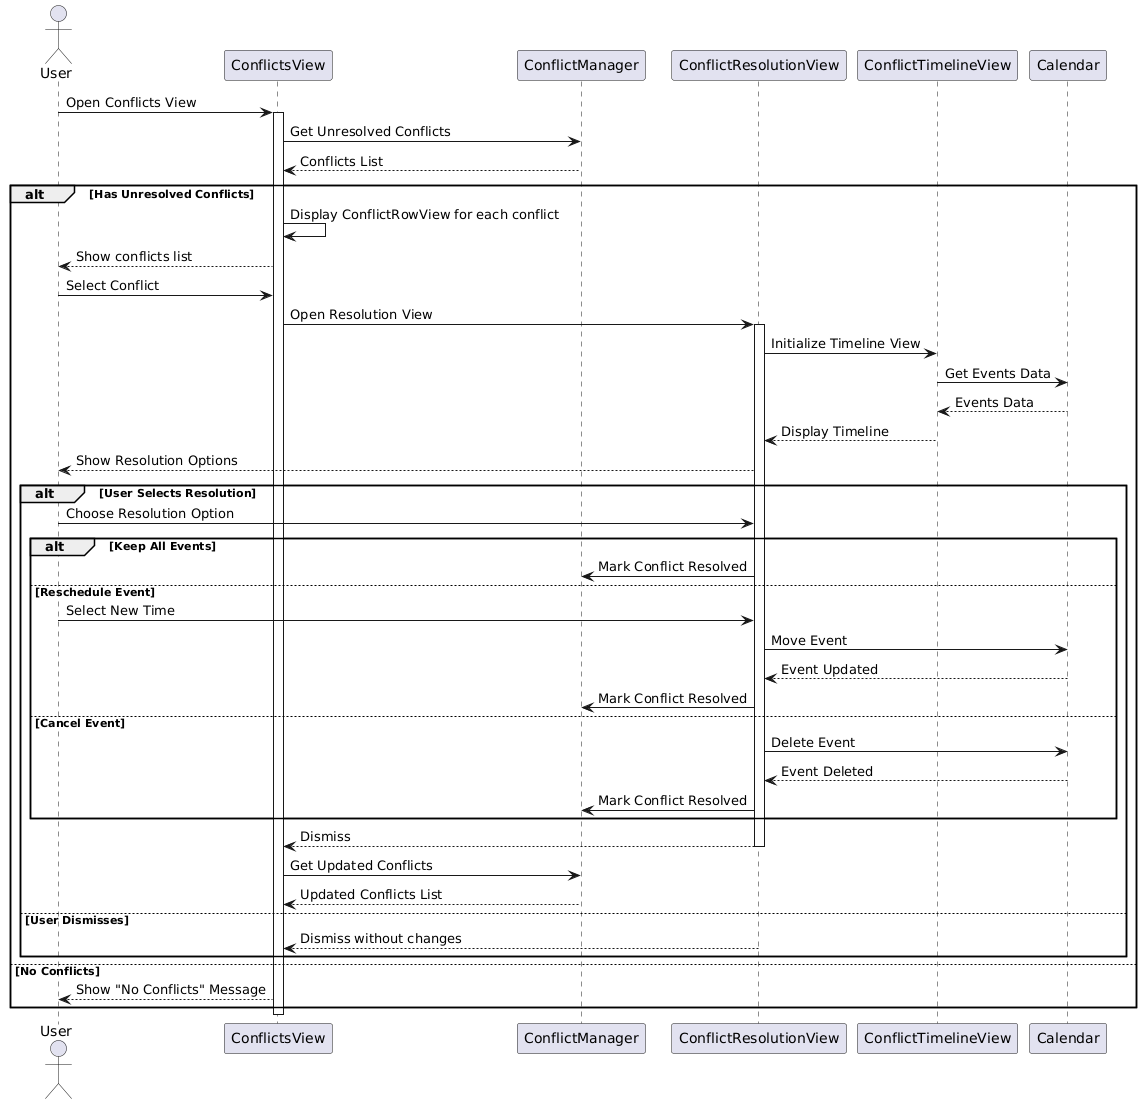
\includegraphics[width=\textwidth]{images/docs/diagrams/sequence-diagrams/all-sequence-diagrams/Manage Scheduling Conflicts.png}
  \caption{Manage Scheduling Conflicts Sequence Diagram}
  \label{fig:seq/manage-scheduling-conflicts}
\end{figure}
\begin{usecase}{Add Event Manually}
    \ucbasicinfo{High}{Regular}
    \ucshortdescription{This UC allows users to add events manually }
    \uctrigger{The user clicks and adds the events.}
    \ucactors{User}{None}
    \ucpreconditions{The user is logged into the application }
    \ucrelationships{N/Al}{N/A}{N/A}
    \ucinputsoutputs{
      \begin{itemize}
        \item \textbf{Event Name} (Source: User)
        \item \textbf{Event Location} (Source: User)
        \item \textbf{Event Date (Start and End)} (Source: User)
        \item \textbf{Event Time (Start and End)} (Source: User)
        \item \textbf{Event Description} (Source: User)
        \item \textbf{Notifications/Reminders} (Source: User)
      \end{itemize}
    }{
      \begin{itemize}
        \item \textbf{The event is displayed on the calendar with its details and duration
        } (Destination: Calendar)
      \end{itemize}
    }
    \ucmainflow{
      \begin{enumerate}
        \item The name of the event (e.g., ``Meeting with Client'')
          \ucinfo{Event is saved and displayed on the user’s calendar}
        \item The start and end time of the event.
          \ucinfo{The system displays the event in the correct time slot with its duration, while checking for conflicts and scheduling notifications}
        \item The User optionally adds a description
          \ucinfo{The system stores and displays description of the event.}
        \item Set reminders for the event.
          \ucinfo{Notification or reminder set for the event}
      \end{enumerate}
    }
    \ucalternateflows{
      \begin{enumerate}
        \item User clicks on a date on the calendar to bring up a popup with event fields and the date is pre-filled. 
        \item	The user can add a different color for the events.
      \end{enumerate}
    }
    \ucexceptions{
      \begin{itemize}
        \item Invalid date and time format\
        \item The event's start and end times conflict with an existing event
        \item The user attempts to save the event without filling in mandatory fields
      \end{itemize}
    }
    \ucconclusion{The UC ends when the event has been successfully added to the calendar, and the user sees it displayed.}
    \ucpostconditions{The event is successfully added to the calendar, visible in the correct time slot, and notifications are set as per user preferences}
    \ucspecialrequirements{The interface must be simple and allowing users to input events with less efforts.}
\end{usecase}
\begin{usecase}{View Integrated Calendar}
  \ucbasicinfo{High}{Regular}
  \ucshortdescription{Allows users to view their integrated calendar}
  \uctrigger{User selects the option to view the integrated calendar.}
  \ucactors{User}{None}
  \ucpreconditions{User must be logged into the system.}
  \ucrelationships{N/A}{N/A}{N/A}
  \ucinputsoutputs{
    \begin{itemize}
      \item \textbf{Integrated calendar} (Source: System)
    \end{itemize}
  }{
    \begin{itemize}
      \item \textbf{Integrated calendar} (Destination: App)
    \end{itemize}
  }
  \ucmainflow{
    \begin{enumerate}
      \item The user clicks on the integrated calendar.
            \ucinfo{The system displays the all integrated calendars and it's events}
    \end{enumerate}
  }
  \ucconclusion{User successfully views their integrated calendar with all the events.}
  \ucpostconditions{The integrated calendar is displayed}
  \ucspecialrequirements{N/A}
  \ucbusinessrules{
    \begin{itemize}
      \item \textbf{Events must be displayed according to user preferences .}
    \end{itemize}
  }
\end{usecase}

\begin{figure}[!h]
  \centering
  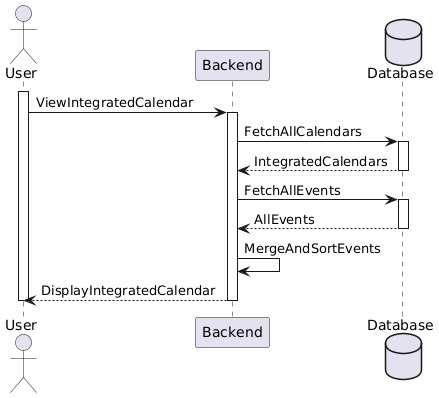
\includegraphics[width=\textwidth]{images/docs/diagrams/sequence-diagrams/all-sequence-diagrams/View Integrated Calendar.png}
  \caption{View Integrated Calendar Sequence Diagram}
  \label{fig:seq/view-integrated-calendar}
\end{figure}

The "View Integrated Calendar Sequence Diagram", shown in \textbf{Figure~\ref{fig:seq/view-integrated-calendar}}, demonstrates the process of presenting a unified view of all connected calendars to the user. The sequence begins when the user initiates a ViewIntegratedCalendar gRPC call to access their comprehensive calendar view.

The Backend executes a two-phase data retrieval process:
\begin{enumerate}
  \item First queries the Database via FetchAllCalendars to retrieve all calendar sources connected to the user's account
  \item Then executes FetchAllEvents to gather events from all calendars
\end{enumerate}

After data retrieval, the Backend performs critical processing:
\begin{itemize}
  \item Merges events from different calendar sources
  \item Sorts events chronologically
  \item Applies user preferences for event display
\end{itemize}

Finally, the Backend returns the processed calendar data through the gRPC channel as DisplayIntegratedCalendar response. This unified view ensures users can efficiently manage their schedule across all connected calendars, maintaining consistency with user preferences while providing a comprehensive overview of all commitments.
\begin{usecase}{Configure Daily Routine}
    \ucbasicinfo{HIGH}{Regular}
    \ucshortdescription{The use case starts when the user initiates the configuration or editing of their daily routine in the app.}
    \uctrigger{The user selects the``Daily Routine'' feature to configure repetitive tasks like waking up, exercise, meals, and sleeping time.}
    \ucactors{User}{None}
    \ucpreconditions{The user is logged into the application }
    \ucrelationships{N/Al}{N/A}{N/A}
    \ucinputsoutputs{
      \begin{itemize}
        \item \textbf{Routine tasks (e.g., wake up, jog, meals, bath time, sleep)} (Source: User)
        \item \textbf{Start and end times for each task.} (Source: User)
        \item \textbf{Recurrence pattern (daily, weekdays, weekends, etc)} (Source: User)
        \item \textbf{Notifications or reminders (e.g., alarms for specific tasks).} (Source: User)
      \end{itemize}
    }{
      \begin{itemize}
        \item \textbf{The daily routine is added to the calendar with all configured tasks displayed as recurring events.} (Destination: Calendar)
      \end{itemize}
    }
    \ucmainflow{
      \begin{enumerate}
        \item The user adds Daily tasks (wake up, meals, sleep, etc.)
          \ucinfo{Routine tasks are added to the calendar.}
        \item The start and end time of the event.
          \ucinfo{The system displays the event in the correct time slot with its duration, while checking for conflicts and scheduling notifications}
      \end{enumerate}
    }
    \ucalternateflows{
      \begin{enumerate}
        \item The user clicks on the calendar, the system displays the daily routine tasks.
      \end{enumerate}
    }
    \ucexceptions{
      \begin{itemize}
        \item Conflict with tasks
      \end{itemize}
    }
    \ucconclusion{Configuring a daily routine enables users to block out dedicated time for recurring tasks.}
    \ucpostconditions{The daily routine is successfully configured and integrated into the calendar, with appropriate visual indicators and reminders.}
    \ucspecialrequirements{The interface must be simple and allowing users to have the daily routines Throughout.}
\end{usecase}
\begin{usecase}{Schedule Prayer Times}
    \ucbasicinfo{High}{Regular}
    \ucshortdescription{Allows users to create, edit, and manage their prayer time schedules.}
    \uctrigger{User selects the option to schedule prayer times.}
    \ucactors{User}{None}
    \ucpreconditions{User must be logged into the system.}
    \ucrelationships{N/A}{N/A}{N/A}
    \ucinputsoutputs{
      \begin{itemize}
        \item \textbf{User's prayer time details} (Source: user)
        \item \textbf{(date, time)}
      \end{itemize}
    }{
      \begin{itemize}
        \item \textbf{Confirmation of scheduled prayer times, calendar entries.}
      \end{itemize}
    }
    \ucmainflow{
      \begin{enumerate}
        \item User navigates to the prayer scheduling page.
          \ucinfo{User is presented with a form to enter prayer times. Display of the scheduling interface.}
        \item User inputs prayer time details.
          \ucinfo{Input fields for time, date, and prayer type. User's input is captured for validation.}
        \item User saves the schedule.
          \ucinfo{System checks for valid input. Confirmation message displayed.}
        \item System confirms schedule creation.
          \ucinfo{User receives a notification. Scheduled prayer times are saved in the system.}
      \end{enumerate}
    }
    \ucalternateflows{
      \begin{itemize}
        \item If input is invalid, display error messages.
      \end{itemize}
    }
    \ucexceptions{
      \begin{itemize}
        \item If there's a system error, display a relevant error message.
      \end{itemize}
    }
    \ucpostconditions{The system generates calendar entries for the scheduled prayer times.}
    \ucspecialrequirements{The system must support notifications for prayer times.}
    \ucconclusion{User's prayer times are successfully scheduled.}
    \ucbusinessrules{
      \begin{itemize}
        \item Prayer times must be within valid time ranges.
      \end{itemize}
    }
\end{usecase}
\begin{usecase}{Receive Event Notifications}
  \ucbasicinfo{High}{Regular}
  \ucshortdescription{Users receive notifications about upcoming events.}
  \uctrigger{The UC is triggered when the choosen time of an event's reminder has arrived}
  \ucactors{User}{None}
  \ucpreconditions{User must be logged into the system and set a reminder of the specific event.}
  \ucrelationships{N/A}{N/A}{N/A}
  \ucinputsoutputs{
    \begin{itemize}
      \item \textbf{Time of the event reminder} (Source: User)
    \end{itemize}
  }{
    \begin{itemize}

      \item \textbf{Notifications sent to users.} (Destination: System)
    \end{itemize}
  }
  \ucmainflow{
    \begin{enumerate}
      \item The system checks the alarms set for every event.
            \ucinfo{The system checks every 1 minute for set alarms for every event.}
      \item Notifications sent to users.
            \ucinfo{The user is reminded about the event by sending the notification}
    \end{enumerate}
  }
  \ucalternateflows{
    \begin{itemize}
      \item \textbf{If user denys the access to the notification the notifications are not sent.}
    \end{itemize}
  }
  \ucexceptions{
    \begin{itemize}
      \item \textbf{Netwok issue}
    \end{itemize}
  }
  \ucconclusion{The system checks for set alarm every 1 minute and if the event is detected the system sends the notification.}
  \ucpostconditions{Notifications are sent.}
  \ucspecialrequirements{Notification permission.}
  \ucbusinessrules{The system has to check every minute for the set alarm.
  }
\end{usecase}

\begin{figure}[!h]
  \centering
  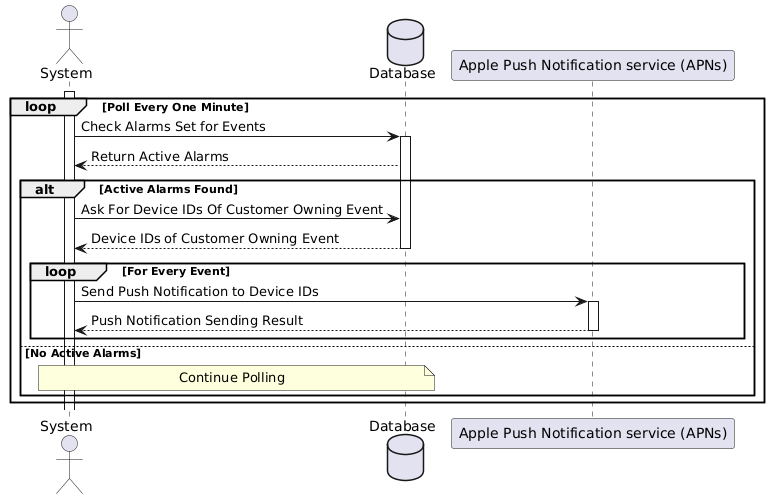
\includegraphics[width=\textwidth]{images/docs/diagrams/sequence-diagrams/all-sequence-diagrams/Receive Event Notifications.png}
  \caption{Receive Event Notifications Sequence Diagram}
  \label{fig:seq/receive-event-notifications}
\end{figure}

The ``Receive Event Notifications Sequence Diagram'', shown in \textbf{Figure~\ref{fig:seq/receive-event-notifications}}, illustrates Jadwal's continuous event notification monitoring and delivery system. The sequence operates in a continuous polling loop that executes every minute, ensuring timely notification delivery for all scheduled events.

The polling process consists of several key steps:
\begin{enumerate}
  \item The System queries the Database for active alarms through regular checks
  \item For each batch of active alarms found:
        \begin{itemize}
          \item Retrieves associated device IDs for notification targets
          \item Iterates through each event requiring notification
          \item Dispatches push notifications via Apple Push Notification service (APNs)
        \end{itemize}
  \item If no active alarms are found, the system continues its polling cycle
\end{enumerate}

This robust notification system ensures reliable delivery of event reminders while efficiently managing system resources. The one-minute polling interval provides a balance between timely notifications and system performance, while the batch processing of notifications optimizes the interaction with APNs. The system's ability to handle multiple device IDs per user ensures notifications reach users across all their registered devices.

% Bibliography
\bibliography{references}
\bibliographystyle{apalike}

\end{document}